\section{Desarrollo}

Dado el problema del horno, en primer lugar debemos modelarlo. Consideremos la secci\'on horizontal de un horno de acero cil\'indrico como el de la siguiente figura. El sector A es la pared del horno, y el sector B es el interior del mismo, en el cual se funde el acero a temperaturas elevadas. Tanto el borde externo como el borde interno de la pared son circulares con un centro en común. Suponemos que la temperatura del acero dentro del horno es constante e igual a 1500$^{o}$C.

\medskip

Existen sensores ubicados en la parte externa del horno para medir la temperatura exterior. La misma se encuentra habitualmente entre 50$^{o}$C y 200$^{o}$C. El problema que debemos resolver consiste en estimar la isoterma de 500$^{o}$C dentro de la pared del horno. Si esta isoterma est\'a demasiado cerca de la pared externa del horno, existe el riesgo que la integridad estructural del horno este comprometida.

\begin{figure}[ht]
\begin{center}
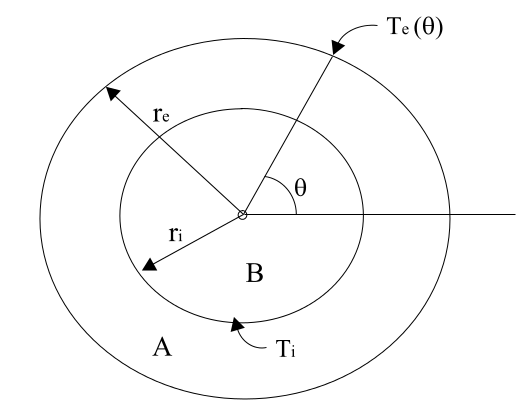
\includegraphics[width=0.4\columnwidth]{catedra/Horno.png}
\caption{Secci\'on circular del horno}
\end{center}
\end{figure}

Sea $r_e \in \mathbb{R}$ el radio exterior de la pared y sea $r_i \in \mathbb{R}$ el radio interior de la pared. Llamemos $T(r,\theta)$ a la temperatura en el punto dado por las coordenadas polares $(r,\theta)$, siendo $r$ el radio y $\theta$ el angulo polar de dicho punto. En el \texttt{estado estacionario}, esta temperatura satisface la ecuación del calor dada por el laplaciano:

\begin{equation}\label{calor}
\frac{\partial^2T(r,\theta)}{\partial r^2}+\frac{1}{r}\frac{\partial T(r,\theta)}{\partial r}+\frac{1}{r^2}\frac{\partial^2T(r,\theta)}{\partial \theta^2} = 0 
\end{equation}

Para resolver esta ecuación de forma numérica, discretizamos la superficie de la pared como en la siguiente figura y luego aproximamos las derivadas parciales utilizando diferencias finitas.

\begin{figure}[ht]
\begin{center}
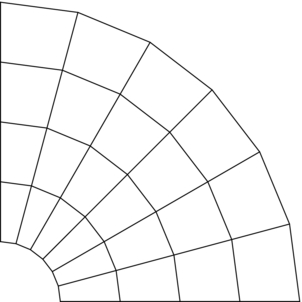
\includegraphics[width=0.2\columnwidth]{catedra/disc.png}
\caption{Discretización de la pared del horno.}
\end{center}
\end{figure}

\begin{equation}
\frac{\partial^2T(r,\theta)}{\partial r^2}(r_j,\theta_k) \cong \frac{t_{j-1,k}-2t_{jk}+t_{j+1,k}}{(\Delta r)^2}
\end{equation}

\begin{equation}
\frac{\partial T(r,\theta)}{\partial r}(r_j,\theta_k) \cong \frac{t_{j,k}-t_{j-1,k}}{\Delta r}
\end{equation}

\begin{equation}
\frac{\partial^2T(r,\theta)}{\partial \theta^2}(r_j,\theta_k) \cong \frac{t_{j,k-1}-2t_{jk}+t_{j,k+1}}{(\Delta \theta)^2}
\end{equation}

Reemplazando la aproximación numérica en el laplaciano y el radio por su respectiva discretización obtenemos:
\begin{equation}\label{calor}
\frac{t_{j-1,k}-2t_{jk}+t_{j+1,k}}{(\Delta r)^2}
+ \frac{1}{r_j}
\frac{t_{j,k}-t_{j-1,k}}{\Delta r}
+
\frac{1}{r_j^2}
\frac{t_{j,k-1}-2t_{jk}+t_{j,k+1}}{(\Delta \theta)^2} = 0 \nonumber
\end{equation}

Donde $r_j = r_i + j \times \Delta r$, $\Delta r = \frac{(r_e - r_i)}{m}$ y $\Delta \theta = \frac{2\pi}{n}$.

De esta manera aproximamos de forma discreta la ecuación diferencial dada por el laplaciano.


Si llamamos $T_i \in \mathbb{R}$ a la temperatura en el interior del horno (sector B) y $T_e : [0,2\pi] \rightarrow \mathbb{R}$ a la función de temperatura en el borde exterior del horno (de modo tal que el punto $(r_e,\theta)$ tiene temperatura $T_e(\theta)$), entonces tenemos que

\begin{equation}
T(r,\theta) = T_i \;\;\;\;\;para\;todo\;punto\;(r,\theta)\;con\;r\leq r_i
\end{equation}
\begin{equation}
T(r_e,\theta) = T_e(\theta) \;\;\;\;\;\;para\;todo\;punto\;(r_e,\theta)
\end{equation}

\subsection{Discretización}

Para resolver este problema computacionalmente, discretizamos el dominio del problema (el sector A) en coordenadas polares. Consideramos una partici\'on $0 = \theta_0 < \theta_1 < ... < \theta_n = 2\pi$ en $n$ \'angulos discretos con $\theta_k-\theta_{k-1} = \Delta\theta$ para $k = 1,...,n$, y una partici\'on $r_i = r_0 < r_1 < ... < r_m = r_e$ en $m+1$ radios discretos con $r_j - r_{j-1} = \Delta r$ para $j = 1,...,m$.

De esta manera, terminamos con un sistema de $(m+1)*n$ ecuaciones lineales, que puede ser experesado como $Ax = b$. Para cada temperatura $t_{j,k}$, tendremos un laplaciano. Esto no sucede con los valores de las temperaturas en las puntas, donde ya a priori sabemos el valor final $t_i$ y $t_e(\theta)$. Estas temperaturas en las puntas formaran parte del vector de valores independientes b al armar el sistema, al que le corresponde un canónico. La discretización muchas veces depende de los valores anteriores y posteriores, por lo que hay que tener cuidado de no caer en uno de estos casos borde al formular el sistema.

\subsection{Sistema Lineal}
Para formular el sistema lineal, en primer lugar debemos despejar cada una de las variables $t_{j,k}$ de la aproximación discreta del laplaciano:

\begin{equation}\label{calor}
\frac{t_{j-1,k}-2t_{j,k}+t_{j+1,k}}{(\Delta r)^2}
+ \frac{1}{r_j}
\frac{t_{j,k}-t_{j-1,k}}{\Delta r}
+
\frac{1}{r_j^2}
\frac{t_{j,k-1}-2t_{j,k}+t_{j,k+1}}{(\Delta \theta)^2} = 0 \nonumber
\end{equation}

Reescribiendo:

\begin{equation}
\alpha_{j,k} \times t_{j,k} + \alpha_{j-1,k} \times t_{j-1,k} + \alpha_{j+1,k} \times t_{j+1,k} + \alpha_{j,k+1} \times t_{j,k+1} + \alpha_{j,k-1} \times t_{j,k-1} = 0 \nonumber
\end{equation}

Donde:

\begin{equation}
\alpha_{j,k} = \frac{-2}{(\Delta r)^2} + \frac{1}{r_j \times \Delta r} + \frac{-2}{r_j^2 \times (\Delta \theta)^2}
\end{equation}

\begin{equation}
\alpha_{j,k+1} = \frac{1}{r_j^2 \times (\Delta \theta)^2}
\end{equation}

\begin{equation}
\alpha_{j,k-1} = \frac{1}{r_j^2 \times (\Delta \theta)^2}
\end{equation}

\begin{equation}
\alpha_{j+1,k} = \frac{1}{(\Delta r)^2}
\end{equation}

\begin{equation}
\alpha_{j-1,k} = \frac{1}{(\Delta r)^2} - \frac{1}{r_j \times \Delta r}
\end{equation}

%\vspace{5mm}

\subsubsection{Matriz del sistema}

Con las ecuaciones \textit{(7)-(11)} armamos la matriz del sistema, en donde los coeficientes ser\'an los $\alpha$ anteriores, expresando en cada fila su valor para cada temperatura. Hay que tener en cuenta que en todas las ecuaciones habr\'a un $\alpha$ para cada uno de los $t_{j,k}$, valiendo $0$ en aquellos casos en que no aparezca dicha incógnita, $1$ en caso de ser $t_i$ o $t_e{\theta}$, o en su defecto $\alpha$ como se han definido en el desarrollo anterior.

Por cuestiones de optimizaci\'on organizamos la matriz con el orden de sus columnas (inducidas por los $t_{k,j}$), de acuerdo al orden de aparici\'on impartido por el recorrido de $\theta_0$ a $\theta_{n-1}$ (variando el radio luego de cada vuelta) desde $r_i$ hasta $r_e$ inclusive.
\\
Gráficamente dicha matriz queda definida de la siguiente forma:
\\

$
\hspace{3.2cm}
     \begin{pmatrix}
      \alpha_{0,0} & \alpha_{0,1} & \cdots & \alpha_{0,(m+1)(n-1)} \\
      \alpha_{1,0} & \alpha_{1,1} & \cdots & \alpha_{1,(m+1)(n-1)} \\
      \vdots  & \vdots  & \ddots & \vdots \\
      \vdots  & \vdots  &        & \vdots \\
      \vdots  & \vdots  &        & \vdots \\
      \vdots  & \vdots  &        & \vdots \\
      \alpha_{(m+1)(n-1),0} & \alpha_{(m+1)(n-1),1} & \cdots & \alpha_{(m+1)(n-1),(m+1)(n-1)} 
     \end{pmatrix}
$
\\
\\
\\
Notese que la indexaci\'on de los coeficientes empieza en $0$, en vez de en $1$ como es habitual; el motivo es el de generar una mayor cohesi\'on con la idexaci\'on de las temperaturas, que a su vez, son indexadas de acuerdo a los $r_i$ y los $\theta_i$ correspondientes (indexados efectivamente desde el $0$).

Ahora bien como las primeras y \'ultimas $n$ filas corresponden al radio interior y exterior respectivamente, sabemos que en ese rango $\alpha_{jj} = 1$ y $\alpha_{ji} = 0, \forall j \neq i$. Lo que nos genera una matriz identidad de $n*n$ en las esquinas superior izquierda e inferior derecha; dando adem\'as a la matriz del sistema la condici\'on de matriz \textit{banda}.
\\
\\

$
\hspace{1.3cm}
     \begin{pmatrix}
      1 & 0 & \cdots & 0 & \cdots & 0 & 0 & \cdots & 0 \\
      0 & \ddots & 0 & \vdots & \cdots & \vdots & \vdots & \ddots & \vdots \\   
      \vdots  & 0  & 1 & 0 & \cdots & 0 & 0 & \cdots & 0 \\
      \alpha_{n-2,0} & \cdots & \cdots & \alpha_{n-2,n-2} & \cdots & \alpha_{n-2,(m+1)(n-1)-n} & \cdots & \cdots & \alpha_{n-2,..} \\
      \vdots  & \ddots  &  & \vdots & \cdots & \vdots &  & \ddots & \vdots \\        
      \alpha_{....,....} &  &\ddots & \alpha_{(m+1)(n-1)-n, n-2} & \cdots & \alpha_{(m+1)n-n,(m+1)(n-1)-n} & & & \alpha_{....,....}  \\
      0 & \cdots & 0 & 0 & \cdots & 0 & 1 & 0 & \cdots  \\
      \vdots & \ddots & \vdots & \vdots & \cdots & \vdots & 0 & \ddots & 0 \\
      0 & \cdots & 0 & 0 & \cdots  & 0 & \cdots & 0 & 1 
     \end{pmatrix}
$

\vspace{4mm}
Si bien no se muestra explicitamente en la figura, para sistemas lo suficientemente grandes se podr\'a apreciar como debajo de la $Id$ superior izquierda y arriba de la $Id$ inferior derecha, se generan submatrices diagonales que estrecharan la anchura de la banda, dejandonos una matriz \textit{banda-n}. 

\iffalse
\subsubsection{Métodos de resolución}


\subsubsection{Eliminaci\'on Gaussiana}

\underline{Eliminaci\'on Gaussiana}
\\

Este metodo consiste en convertir a la matriz de entrada en una matriz \testit{equivalente} que cumple con la condici\'on de triangular superior. Esta en particular es el resultado de la composici\'on de una serie de matrices elementales, que consiguen realizar una serie de conmutaciones, sumas y multiplicaciones (por escalares). Dicho composici\'on se puede realizar por el siguiente algoritmo iterativo.
\begin{itemize}
\item Para $i = 1,...,n-1$
\begin{itemize}
\item Si $a_{ii} = 0$ intercambio $Fila_i$ con $Fila_j$ tal que $a_{ji} \neq 0, j<i$ 
\item Para $j = i+1,...,n$
\begin{itemize}
\item $m_{ji} = \frac{\alpha_{ji}}{\alpha_{ii}}$
\item $Fila_j = Fila_j - m_{ji}*Fila_i$
\end{itemize}
\end{itemize}
\end{itemize}

\textbf{Agregar pseudo-codigo de la forma en la que armamos el sistema. Hablar de EG, LU y su respectiva complejidad.}
\fi

\subsection{Isoterma}
Una vez que resolvamos el sistema lineal, debemos buscar la isoterma. Dado que es una aproximación discreta, es muy probable que no encontremos valores de temperatura iguales a la curva de nivel. Por lo tanto debemos tener cierta tolerancia de error, o hasta interpolar de alguna manera las curvas de nivel adyacentes en la discretización. Es decir, debemos definir algún criterio de búsqueda sobre el vector $b$. Nuestros criterios de búsqueda se basaran en el supuesto de que a medida que nos alejamos del centro del horno en \texttt{estado estacionario}, las temperaturas serán menores. Una consideración sumamente importante en el contexto de nuestro problema: intentaremos buscar métodos que sean pesimistas, es decir, que sigan el principio de prudencia. Esto significa que nuestros algoritmos intentaran ubicar la aproximación de la isoterma mas cerca de la pared del horno de lo que efectivamente esta, para poder evaluar de forma certera si el horno es estructuralmente estable o no.

\subsubsection{Algoritmo: Primer menor}

El primer criterio de búsqueda consiste en tomar el primer valor de temperatura menor al que estamos buscando para cada angulo en la discretización. Esto se puede ver en el siguiente pseudo-código:

\begin{algorithmic}
\Procedure{Lower}{}
\State posicion $\gets$ Vector($\vert$angulos$\vert$)
\For{i \textbf{in} angulos}
    \State $posicion_i$ $\gets$ \texttt{primer radio con temperatura menor a la isoterma}
\EndFor
\Return{posicion}
\EndProcedure
\end{algorithmic}

\subsubsection{Algoritmo: Promedio pesado}

Este criterio buscara ubicar la isoterma de forma inteligente, buscando el valor mayor y menor entre los que se ubica la isoterma y haciendo un promedio pesado. Esto se puede ver en el siguiente pseudo-código:

\begin{algorithmic}
\Procedure{Weighted}{}
\State posicion $\gets$ Vector($\vert$angulos$\vert$)
\For{i \textbf{in} angulos}
    \State a $\gets$ \texttt{ultimo radio con temperatura mayor a la isoterma}
    \State b $\gets$ \texttt{primer radio con temperatura menor a la isoterma}
    \State $posicion_i$ $\gets$ a + $\frac{temp(a)-temp(b)}{isoterma}(b-a)$
\EndFor
\Return{posicion}
\EndProcedure
\end{algorithmic}

\subsection{Propiedades del sistema}
Como ya se ha visto en la materia, no es posible aplicar los métodos propuestos para la resoluci\'on a cualquier sistema de ecuaciones. Por ello deberemos demostrar la siguiente proposici\'on.

\begin{proposition}
Sea $A \in \mathbb{R}^{n \times n}$ la matriz obtenida para el sistema definido por (1)-(6). Demostrar que es posible
aplicar Eliminaci\'on Gaussiana sin pivoteo.
\end{proposition}

Con este proposito es que analizaremos algunas propiedades que satisface nuestra matriz, y como a\'un bajo el proceso de Eliminaci\'on Gaussiana, se mantienen fieles e invariantes.
\\
\\
\underline{\textit{A} es d.d.(no estricta)}
\\
\\
Demostremos primero que la matriz $A$ del sistema lineal, definida como antes, cumple la propiedad de ser diagonal dominante (no estricta).

Esto en nuestro caso es pedir que:

\begin{equation}
 \left | \alpha_{jj} \right | \geq \sum_{k=0,k \neq j}^{(m+1)(n-1)} \left | \alpha_{jk} \right |, \forall j \in \{ 0,...,(m+1)(n-1)\}
\end{equation}

En el caso de que $j \in \{0,...,n-1\} \cup \{(m+1)(n-1)-n,...,(m+1)(n-1))\}$, es decir, que se trate de las primeras o \'ultimas $n$ filas, $(12)$ es satisfecha trivialmente, pues  $\left | \alpha_{jj} \right | = 1 \geq \sum_{k=0,k \neq j}^{(m+1)(n-1)} \left | \alpha_{jk} \right | =  \underbrace{0+ \ldots +0}_{(m+1)(n)} = 0$ pues $\alpha_{jk_{k\neq j}}=0 $ 
\\
\\
Nos queda ver el caso contrario. Para ello debemos desarrollar la sumatoria y despejar los $\alpha_{jk}$ mediante $(7)...(11)$, de los cuales los siguientes 5 se\'an los \'unicos $\alpha_{jk}$ distintos de $0$.
\\
De este caso, en particular llegaremos a una equivalencia.

\begin{equation}
 \left | \alpha_{jj} \right | = \left | \alpha_{j+1k} \right | + \left | \alpha_{j-1k} \right | + \left | \alpha_{jk-1} \right | + \left | \alpha_{jk+1} \right |
\end{equation}

\begin{equation}
 \left | \frac{-2}{(\Delta r)^2} + \frac{1}{r_j \times \Delta r} + \frac{-2}{r_j^2 \times (\Delta \theta)^2} \right | = \left | \frac{1}{(\Delta r)^2} \right | + \left | \frac{1}{(\Delta r)^2} - \frac{1}{r_j \times \Delta r} \right | + \left | \frac{1}{r_j^2 \times (\Delta \theta)^2} \right | + \left | \frac{1}{r_j^2 \times (\Delta \theta)^2} \right |
\end{equation}

\begin{equation}
 \left | -\left ( \frac{-2}{(\Delta r)^2} + \frac{1}{r_j \times \Delta r} + \frac{-2}{r_j^2 \times (\Delta \theta)^2} \right ) \right | = \left | \frac{1}{(\Delta r)^2} \right | + \left | \frac{1}{(\Delta r)^2} - \frac{1}{r_j \times \Delta r} \right | + \left | \frac{2}{r_j^2 \times (\Delta \theta)^2} \right | 
\end{equation}

\begin{equation}
 \left | \frac{1}{(\Delta r)^2} + \underbrace{\frac{1}{(\Delta r)^2} - \frac{1}{r_j \times \Delta r}}_{ \geq 0} + \frac{2}{r_j^2 \times (\Delta \theta)^2} \right | = \left | \frac{1}{(\Delta r)^2} \right | + \left | \frac{1}{(\Delta r)^2} - \frac{1}{r_j \times \Delta r} \right | +  \left | \frac{2}{r_j^2 \times (\Delta \theta)^2} \right |
\end{equation}

\begin{equation}
 \left | \frac{1}{(\Delta r)^2} \right | + \left | \frac{1}{(\Delta r)^2} - \frac{1}{r_j \times \Delta r} \right | + \left | \frac{2}{r_j^2 \times (\Delta \theta)^2} \right | = \left | \frac{1}{(\Delta r)^2} \right | + \left | \frac{1}{(\Delta r)^2} - \frac{1}{r_j \times \Delta r} \right | +  \left | \frac{2}{r_j^2 \times (\Delta \theta)^2} \right | \qed
\end{equation}
\\
\\
Con este resultado probamos que la matriz inicial $A$ es diagonal dominante (no estricta), ahora nos toca ver que el algoritmo preserva esta propiedad a lo largo de cada iteraci\'on. Naturalmente lo probaremos por inducci\'on.
\\
\\
* De ahora en mas notaremos como $\alpha_{jk}^{(i)}$ al coeficiente situado en la posición de $\alpha_{jk}$ en  $A$, de la matriz $A^{(i)}$ obtenida como resultado tras aplicar las primeras $i-1$ iteraciones de la Eliminaci\'on Gaussiana. \textit{Ej: $\alpha_{jk}^{(2)}$ alude al nuevo $\alpha_{jk}$ obtenido tras triangular s\'olo la seccion de la primera columna.}
\\  
\\
\underline{Veamos el caso base:}
\\
\\
Siendo $A$ $d.d.$ (no estricta), probemos que $\left | \alpha_{jj}^{(2)} \right | \geq \sum_{k=0,k \neq j}^{(m+1)(n-1)} \left | \alpha_{jk}^{(2)} \right |, \forall j \in \{1,...,(m+1)(n-1)\}$
\\
\\
\begin{equation}
\alpha_{jk}^{(2)} =  \alpha_{jk} - \frac{\alpha_{0k}}{\alpha_{00}}\alpha_{j0}
\end{equation}

\begin{equation}
\sum_{k=1,k \neq j}^{(m+1)(n-1)} \left | \alpha_{jk}^{(2)} \right | = \sum_{k=1,k \neq j}^{(m+1)(n-1)} \left | \alpha_{jk} - \frac{\alpha_{0k}}{\alpha_{00}}\alpha_{j0} \right | \leq \sum_{k=1,k \neq j}^{(m+1)(n-1)} \left | \alpha_{jk} \right | + \sum_{k=1,k \neq j}^{(m+1)(n-1)} \left | \frac{\alpha_{0k}\alpha_{j0}}{\alpha_{00}} \right | 
\end{equation}

\begin{equation}
\leq \left | \alpha_{jj} \right | - \left | \alpha_{j0} \right | + \frac{\left | \alpha_{j0} \right |}{\left | \alpha_{00} \right |}\left(\left | \alpha_{00} \right | - \left | \alpha_{0j} \right | \right) \leq \left | \alpha_{jj} \right | - \frac{\left | \alpha_{j0} \right | \left |\alpha_{0j} \right | }{ \left | \alpha_{00} \right | } \leq \left | \alpha_{jj} - \frac{\alpha_{j0}\alpha_{0j}}{\alpha_{00}} \right | = \left | \alpha_{jj}^{(2)} \right |
\end{equation}
\\
\\
\underline{Paso inductivo:}
\\
\\
Por hipotesis tenemos que $\left | \alpha_{jj}^{(i)} \right | \geq \sum_{k=0,k \neq j}^{(m+1)(n-1)} \left | \alpha_{jk}^{(i)} \right |, \forall j \in \{i-2,...,(m+1)(n-1)\}$ para las primeras $i-1$ iteraciones.
\\
\\
Queremos ver que: $\left | \alpha_{jj}^{(i+1)} \right | \geq \sum_{k=0,k \neq j}^{(m+1)(n-1)} \left | \alpha_{jk}^{(i+1)} \right |, \forall j \in \{i-1,...,(m+1)(n-1)\}$
\\
\\
\begin{equation}
\alpha_{jk}^{(i+1)} =  \alpha_{jk}^{(i)} - \frac{\alpha_{i-2,k}^{(i)}}{\alpha_{i-2,i-2}^{(i)}}\alpha_{j,i-2}^{(i)}
\end{equation}
\\
\begin{equation}
\sum_{k=i-1,k \neq j}^{(m+1)(n-1)} \left | \alpha_{jk}^{(i+1)} \right | = \sum_{k=i-1,k \neq j}^{(m+1)(n-1)} \left | \alpha_{jk}^{(i)} - \frac{\alpha_{i-2,k}^{(i)}}{\alpha_{i-2,i-2}^{(i)}}\alpha_{j,i-2}^{(i)} \right | \leq \sum_{k=i-1,k \neq j}^{(m+1)(n-1)} \left | \alpha_{jk}^{(i)} \right | + \sum_{k=i-1,k \neq j}^{(m+1)(n-1)} \left | \frac{\alpha_{i-1,k}^{(i)}\alpha_{j,i-2}^{(i)}}{\alpha_{i-2,i-2}^{(i)}} \right | 
\end{equation}

\begin{equation}
\stackrel{\text{Por Hip.}}{\leq} \left | \alpha_{jj}^{(i)} \right | - \underbrace{\sum_{k=0,k \neq j}^{i-2} \left | \alpha_{j,k}^{(i)} \right |}_{= 0} + \frac{\left | \alpha_{j,i-2}^{(i)} \right |}{\left | \alpha_{i-2,i-2}^{(i)} \right |}\left(\left | \alpha_{i-2,i-2}^{(i)} \right | - \underbrace{\sum_{k=0,k \neq j}^{i-2} \left | \alpha_{i-2,k}^{(i)} \right |}_{= 0} \right)
\end{equation}

\begin{equation}
\leq \left | \alpha_{jj}^{(i)} \right | - \frac{\left | \alpha_{j,i-2}^{(i)} \right | \left |\alpha_{i-2,j}^{(i)} \right | }{ \left | \alpha_{i-2,i-2}^{(i)} \right | } \leq \left | \alpha_{jj}^{(i)} - \frac{\alpha_{j,i-2}^{(i)}\alpha_{i-2,j}^{(i)}}{\alpha_{i-2,i-2}^{(i)}} \right | = \left | \alpha_{jj}^{(i+1)} \right | \qed
\end{equation}
\\
\\
Finalizada así esta demostraci\'on, sabemos que podemos contar con que tanto la matriz inicial $A$ como $A^{(i)}$, son $d.d.$ (no estricta). Por desgracia, si bien esta hipotesis parece alentadora, es insuficiente para garantizar que a $A$ se le pueda aplicar la Eliminaci\'on Gaussiana sin pivoteo. Esto es así porque $A^{(i)}$ a\'un puede caer en un caso borde, el de tener al $0$ como valor en alguno de los elementos de su diagonal principal, y obviamente a alg\'un otro distinto de $0$ en la parte inferior de su misma columna; lo que induciría a un intercambio de filas (pivoteo).

Teniendo en claro cual es el conflicto al que nos enfrentamos, de ahora en mas, nos enfocaremos en probar que para la matriz $A^{(i)}$ del sistema esta situaci\'on no se nos presenta.
\\
\\
\underline{$A^{(i)}$ no tiene al $0$ en su diagonal}
\\
\\
Para empezar podemos observar que dicha situaci\'on s\'olo podr\'ia suceder en cierta sección conflictiva, en particular sobre la submatriz central que resulta de \textit{recortar} las primeras y \'ultimas $n$ filas y columnas. La razón de esto, es porque las primeras $n$ filas son $\mathit{e}_1$ a $\mathit{e}_n$ ordenadas de manera triangular; de esta forma no solo ese tramo de la diagonal posee todos sus elementos distintos de $0$, sino que adem\'as la Eliminaci\'on Gaussiana triangular\'a la primera sección de $n$ columnas, sin alterar a la sección complementaria; y obviamente sin emplear pivoteo. Analogamente resulta que las \'ultimas $n$ filas son $\mathit{e}_{(m+1)(n-1)-n}$ a $\mathit{e}_{(m+1)(n-1)}$, de nuevo, ordenadas de manera triangular; por lo que al llegar a aquella sección, ya no es necesario seguir transformando la matriz, dado que la obtenida hasta el momento, ya es triangular. Dicho esto, llamemos $A^{(*)}$ a la sección de $A$ delimitara por aquel \textit{recorte}.
\\
\\
Sobre $A^{(*)}$, veremos que se cumple una segunda hipótesis bastante útil, y es que todos los elementos de la diagonal son negativos, y los que no lo son, son $0$ o positivo; 
al menos 1 de ellos es de esta \'ultima forma (ignorando el caso trivial de que $A^{(*)}$ sea de $1x1$).
Para esto basta ver que los \'unicos coeficientes definidos (distinto de $0$) en las filas de $A^{(*)}$ son $\alpha_{jj}, \alpha_{j-1,j}, \alpha_{j+1,j}, \alpha_{j,j-1}, \alpha_{j,j+1}$, donde los \'ultimos tres son cocientes positivos, puesto que s\'olo involucran a $\Delta r$, $\Delta \theta$, y $rj$, como denominador (que son positivos). Y como $rj \times \Delta r > (\Delta r)^{2}$, $\alpha_{j-1,j}$ también es positivo. S\'olo queda analizar si efectivamente $\alpha_{jj}$ es negativo. 
\\
\\
\begin{equation}
\alpha_{jj} = \frac{-2}{(\Delta r)^2} + \frac{1}{r_j \times \Delta r} + \frac{-2}{r_j^2 \times (\Delta \theta)^2} < \frac{-2}{(\Delta r)^2} + \frac{1}{r_j \times \Delta r} < \frac{-2}{r_j \times \Delta r} + \frac{1}{r_j \times \Delta r} = \frac{-1}{r_j \times \Delta r} < 0 \qed
\end{equation}
\\
\\
Con esto, ya podemos justificar porque $A^{(i)}$ no tiene ceros en algún elemento de su diagonal. Usando una obsevaci\'on mas, en la que nos restrigiremos a $A^{(*)}$ e ignoraremos la \'ultima fila (pues ya no necesitamos usar el elemento de su diagonal).
Primero notemos que para cada fila habr\'a un elemento detrás (con respecto al recorrido de un radio en particular) del de la diagonal (el $\alpha_{j,j+1}$), que como ya vimos, es positivo. Al ser este elemento positivo, en la iteraci\'on n\'umero $i$ al elemento $\alpha_{j,j+1}$ se le restar\'a $\alpha_{i,j+1}*\alpha{j,i}*(\alpha_{ii})^{-1}$, que al ser $\alpha_{i,j+1}$ y $\alpha{j,i}$ positivos, y $\alpha_{i,i}$ negativo, $\alpha_{j,j+1}$ no podr\'a hacerse mas chico (pues se le esta restando algo negativo). Habrá que rescatar un caso borde; en el argumento anterior estamos usando que $\alpha_{j,j+1}$ esta situado detrás de $\alpha_{j,j}$, pero esto s\'olo ocurre si $\alpha_{j,j}$ no es el u\'ltimo elemento del \textit{anillo} conformado por el radio $r_{j}$. No obstante habrá otro elemento situado mas hacia atrás (el $\alpha_{j+1,j}$) que corresponde al radio inmediatamente superior, tambi\'en mayor a cero. El \'ultimo caso borde ocurre si ese radio inmediatamente superior es el $r_e$ (que no figura en $A^{(*)}$), pero a esto se le puede restar importancia, pues en ese caso $\alpha_{j,j}$ ser\'a el \'ultimo elemento de la diagonal de $A^{(*)}$. Toda esta descripci\'on de la matriz se ve para un sistema lo suficientemente grande, como su condici\'on de matriz \textit{banda}. 

Ahora por \'ultimo, como sabemos que $A^{(i)}$ es $d.d.$(no estricta) y que adem\'as siempre tiene un elemento positivo en cada fila (ignorando a la \'ultima), $\alpha_{jj}$ jamas podr\'a ser igual $0$, porque ser\'ia equivalente a pedir que todos los elementos de su fila, fueran $0$.

 
